%========================
% Document class and theme
%========================
\documentclass[8pt]{beamer}
\usetheme[progressbar=frametitle]{metropolis}
\setbeamersize{text margin left=10mm, text margin right=10mm}
\usepackage{appendixnumberbeamer} % appendix slide numbering
\setbeamertemplate{theorems}[numbered]

%========================
% Core packages
%========================
\usepackage{amsmath, amsfonts, amssymb, amsthm} % math + theorems
\usepackage{booktabs}        % professional tables
\usepackage{hyperref}        % hyperlinks
\usepackage{xcolor}          % colors
\usepackage{xspace}          % spacing for custom commands

%========================
% Algorithms
%========================
\usepackage{algorithm}
\usepackage{algpseudocode}
\newtheorem{proposition}{Proposition}
\usepackage{bbm}


%========================
% Plots and TikZ
%========================
\usepackage{pgfplots}
\usepgfplotslibrary{dateplot}
\usepackage{tikz}
\usetikzlibrary{positioning}

% ==========================================
% Professional Code Listing Setup
% ==========================================
\usepackage{listings}
\definecolor{codegreen}{rgb}{0,0.6,0}
\definecolor{codegray}{rgb}{0.5,0.5,0.5}
\definecolor{codepurple}{rgb}{0.58,0,0.82}
\definecolor{backcolour}{rgb}{0.95,0.95,0.92}

\lstdefinestyle{mystyle}{
    backgroundcolor=\color{backcolour},   
    commentstyle=\color{codegreen},
    keywordstyle=\color{magenta},
    numberstyle=\tiny\color{codegray},
    stringstyle=\color{codepurple},
    basicstyle=\ttfamily\footnotesize,
    breakatwhitespace=false,         
    breaklines=true,                 
    captionpos=b,                    
    keepspaces=true,                 
    numbers=left,                    
    numbersep=5pt,                  
    showspaces=false,                
    showstringspaces=false,
    showtabs=false,                  
    tabsize=2
}

\lstset{style=mystyle}


%========================
% Custom commands
%========================
\newcommand{\themename}{\textbf{\textsc{metropolis}}\xspace}

%========================
% Custom footline
%========================
\setbeamertemplate{footline}
{%
  \leavevmode%
  \hbox{%
  \begin{beamercolorbox}[wd=.35\paperwidth,ht=2.5ex,dp=1.5ex,center]{author in head/foot}%
    \usebeamerfont{author in head/foot}\insertshortauthor
  \end{beamercolorbox}%
  \begin{beamercolorbox}[wd=.3\paperwidth,ht=2.5ex,dp=1ex,center]{title in head/foot}%
    \usebeamerfont{title in head/foot}\insertshorttitle
  \end{beamercolorbox}%
  \begin{beamercolorbox}[wd=.3\paperwidth,ht=2.5ex,dp=1ex,right]{date in head/foot}%
    \usebeamerfont{date in head/foot}\insertframenumber{} / \inserttotalframenumber
  \end{beamercolorbox}}%
  \vskip0pt%
}

%========================
% Beamer tweaks
%========================
\setbeamertemplate{navigation symbols}{} % remove default navigation symbols


%%%%%%%%%%%%%%%%%%%%%%%%%%%%%%%%%%%%%%%%%%%%%%%%%%%%%%%%%%%%%%%%%%%%
%%%%%%%%%%%%%%%%%%%%%%%%%%%%%%%%%%%%%%%%%%%%%%%%%%%%%%%%%%%%%%%%%%%%
% AQUI SE DEFINEN LAS IMAGENES PARA UTILIZAR DESPUES
%\pgfdeclareimage[interpolate=true, height=7cm,width=16cm]{halton-points}{halton-points}
%\pgfdeclareimage[interpolate=true, height=3cm, width =4cm]
%{serie-petroleo-reducido}{serie-petroleo-reducido}
%\pgfdeclareimage[interpolate=true, height=3cm, width =4cm]{rectangle-triangle}{rectangle-triangle}
%\pgfdeclareimage[interpolate=true, height=3cm, width =4cm]{any-angle}{any-angle}
%\pgfdeclareimage[interpolate=true, height=3cm, width =4cm]{Pythagoras}{Pythagoras}


\title{Chapter 3 - Monte Carlo Methods}
\subtitle{Introduction to Monte Carlo Methods.}
\author{Prof. Alex Alvarez, Ali Raisolsadat}
\institute{School of Mathematical and Computational Sciences \\ University of Prince Edward Island}
\date{} % leave empty or add \today
%\title[Stat 4110]{Stat 4110 Statistical Simulation}
%\subtitle{}
%\author[University of Prince Edward Island]{School of Mathematical and Computational Sciences \\ University of Prince Edward Island}

%========================
% Begin document
%========================
\begin{document}

%-------------------
% Title frame
%-------------------
\maketitle

%-------------------
% Slide 1: Origins of Monte Carlo
%-------------------
\begin{frame}{History of the Monte Carlo Method}
\begin{columns}
    % Left column: history text
    \begin{column}{0.65\textwidth}
        \begin{itemize}
            \item The Monte Carlo method was developed in the 1940s during research for the Manhattan Project.
            \item Mathematician Stanislaw Ulam conceived the idea while recovering from an illness, inspired by thinking about solitaire.
            \item He wondered: \textit{“What is the expected number of winning hands in a game of solitaire?”}
            \item This question led to the use of repeated random sampling to estimate expectations — the foundation of Monte Carlo simulation.
        \end{itemize}
    \end{column}

    % Right column: Ulam picture
    \begin{column}{0.35\textwidth}
        \begin{center}
            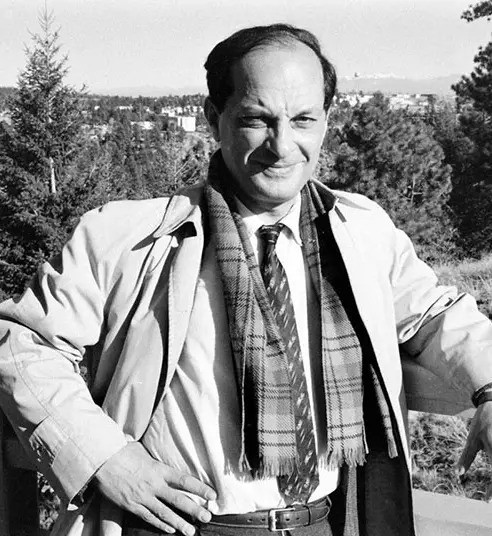
\includegraphics[width=\textwidth]{ulam.jpg} % Replace with actual file
            \\[0.5em]
            \footnotesize Stanislaw Ulam (1909–1984)
        \end{center}
    \end{column}
\end{columns}
\end{frame}

%-------------------
% Slide 2: Early Development
%-------------------
\begin{frame}{Early Development and Implementation}
\begin{columns}
    % Left column: history text
    \begin{column}{0.65\textwidth}
    \begin{itemize}
        \item Ulam proposed using random sampling to solve complex problems in neutron diffusion.
        \item John von Neumann and colleagues formalized the method and implemented it on the ENIAC computer, one of the earliest electronic computers.
        \item The name \textit{“Monte Carlo”} was inspired by the frequent trips of Ulam's uncle to the casino in Monte Carlo, Monaco.
    \end{itemize}
    \end{column}

    % Right column: images
    \begin{column}{0.35\textwidth}
        \begin{center}
        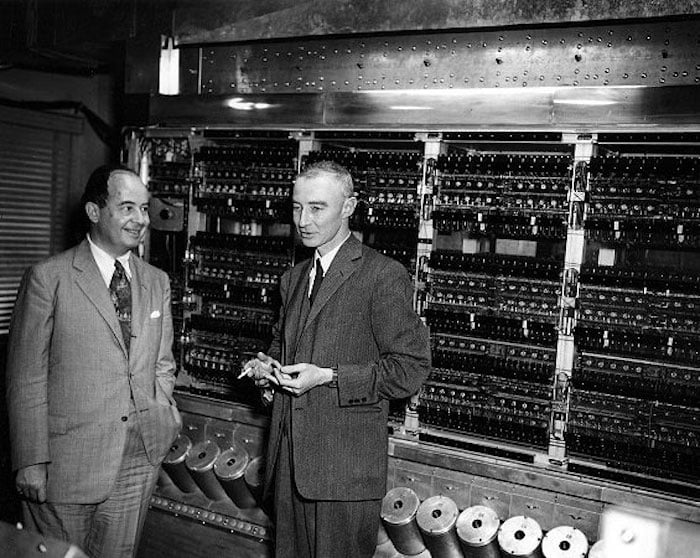
\includegraphics[width=\textwidth]{oppenheimer-neuman-ecp.jpg} % Replace with actual file
        \\[0.5em]
        \footnotesize ENIAC - John von Neumann and Oppenheimer

        \vspace{1em}

        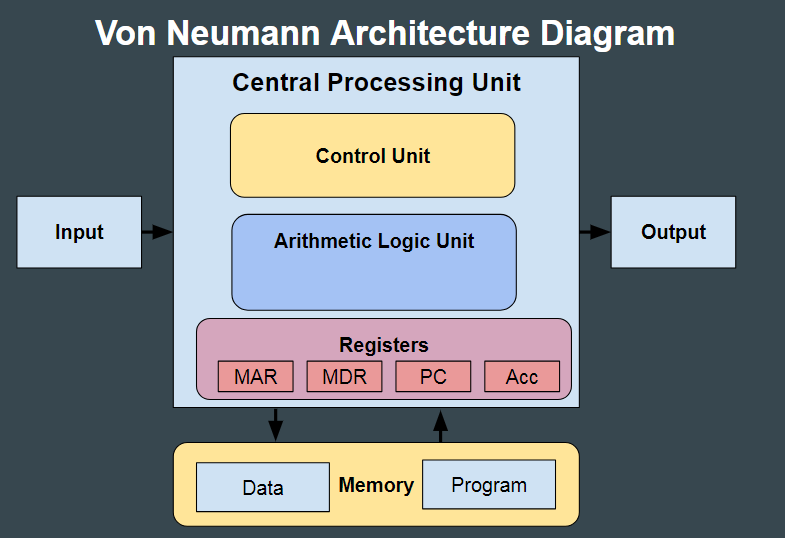
\includegraphics[width=\textwidth]{von-neumann-architecture-gcse-ocr.png} % Replace with actual file
        \\[0.5em]
        \footnotesize Von Neumann architecture
        \end{center}
    \end{column}
\end{columns}
\end{frame}

%-------------------
% Slide 3: Introduction to Monte Carlo Methods
%-------------------
\begin{frame}{Introduction to Monte Carlo Methods}

\begin{itemize}
	\item Monte Carlo methods are a general class of computational algorithms that generate random scenarios to obtain  numerical results.
	\vspace{2mm}
    \item These methods are widely used in statistical physics, computational chemistry, statistical inference, genetics, and finance.
	\vspace{2mm}
    \item The Metropolis algorithm, a key Monte Carlo technique, was named one of the top algorithms of the 20th century by a committee of mathematicians, computer scientists, and physicists.
    \vspace{2mm}
    \item The increasing availability of computational power has greatly expanded the use of Monte Carlo simulations.
    \vspace{2mm}
    \item Monte Carlo methods can be used to solve a variety of mathematical problems. \textbf{In its most basic form, we use it as a numerical integration method} for integrals with no explicit solution. In this course we will also explore other uses of Monte Carlo methods.
\end{itemize}
\end{frame}

%-------------------
% Slide 4: Particle in Random Medium
%-------------------
\begin{frame}[fragile]{Motivation: Particle in a Random Medium}
\begin{itemize}
    \item Consider a particle $(X_t)_{t=1,2,\dots}$ moving in space $\Omega = \mathbb{R}^d$ according to a stochastic model (e.g., random walk, diffusion, or Markov chain). Randomness may arise from the environment ("medium") or from the particle's motion.
    \item \textbf{Absorption rule:} At each time step $t$, the particle can be absorbed with probability $1 - G(X_t)$, where $G: \Omega \to [0,1]$ is the \textbf{survival weight} at location $X_t$.
    \begin{itemize}
        \item $G(x) \approx 1$: safe location (low absorption risk)
        \item $G(x) \approx 0$: high absorption risk (almost surely absorbed)
    \end{itemize}
    \item The survival probability up to time $T$ is
    \begin{equation*}
        \mathbb{P}(\text{not absorbed at time } T) 
        = \mathbb{E}\Big[ \prod_{t=1}^{T} G(X_t) \Big].
    \end{equation*}
\end{itemize}
\end{frame}

%-------------------
% Slide 5: Multiple Particles
%-------------------
\begin{frame}[fragile]{Multiple Particles in a Random Medium}
\begin{itemize}
    \item Suppose we have $n$ independent particles, each evolving over $T$ time steps according to the stochastic model.
    \item Let $X_{i,t}$ denote the position of particle $i$ at time $t$, for $i = 1,\dots,n$ and $t = 1,\dots,T$.
    \item Let $G(X_{i,t})$ denote the survival weight at that position.
    \item The joint survival probability for all particles is
    \begin{equation*}
        \mathbb{P}(\text{all particles survive up to } T)
        = \mathbb{E}\Big[ \prod_{i=1}^{n} \prod_{t=1}^{T} G(X_{i,t}) \Big].
    \end{equation*}
    \item For continuous positions, this is a $(n \cdot T)$-dimensional integral:
    \begin{align*}
        \mathbb{E}\Big[ \prod_{i=1}^{n} \prod_{t=1}^{T} G(X_{i,t}) \Big] 
        = \int \cdots \int \prod_{i=1}^{n} \prod_{t=1}^{T} G(x_{i,t})
        \, p(x_{1,1},\dots,x_{n,T}) \, dx_{1,1} \cdots dx_{n,T}
    \end{align*}
    where $p(\cdot)$ is the joint density of all particle positions.
\end{itemize}
\end{frame}

%\frame
%{

%{\bf Why using Monte Carlo methods in finance?}
%\vspace{3mm}

%Monte Carlo methods can be used to solve many financial problems. Most %applications focus on option pricing or to compute risk measures.
%\vspace{3mm}

%Under some conditions, an option price can be written as a discounted %expected value of the option payoff:

%$$C=e^{-rT}E_Q(\Pi(S_T))$$

%where $Q$ refers to the risk neutral probability and $\Pi(S_T)$ refers to %the option payoff at time $T$.
%\vspace{3mm}

%If we know the probability distribution of $S_T$, then the expression for %$C$ can be written as an integral.
%}

%-------------------
% Slide 6: Computing Expected Values
%-------------------
\begin{frame}{Computing Expected Values}
Let $X=(X_1,X_2,\ldots,X_d)$ be a random vector with joint density $f(x_1,x_2,\ldots,x_d)$ and $g: \mathbb{R}^d \rightarrow \mathbb{R}$. We want to compute:
\begin{equation*}
    E g(X)= \int_{\mathbb{R}^d} g(x)f(x) dx
\end{equation*}

If the integral on the right hand side cannot be solved explicitly, we are only left with numerical methods to get an approximated value of that integral. 

\vspace{3mm}

To simplify the presentation we will assume next that we are in the one-dimensional case ($d=1$) but most results apply also in the multidimensional case.
\end{frame}

%-------------------
% Slide 7: The Law of Large Numbers
%-------------------
\begin{frame}{The Law of Large Numbers}
The main theoretical justification to use Monte Carlo methods is the Law of large numbers:

\vspace{3mm}

{\bf Theorem:} Let be $(X_n)$ independent and identically distributed(i.i.d.) sequence of random variables with 
$E(X_n)=\mu$, $Var(X_n)=\sigma^2$ (both finite). Then we have:\\
\begin{equation*}
\overline{X}_n=\frac{1}{n} \sum_{i=1}^n X_i\rightarrow \mu
\end{equation*}
with probability 1.
\end{frame}

%-------------------
% Slide 8: The Law of Large Numbers Consequences
%-------------------
\begin{frame}{Consequences}
If $X_1,X_2,\ldots,X_n$ is a simulated random sample with the same probability law as $X$  \\
\begin{equation*}
    \frac{1}{n} \sum_{j=1}^n g(X_j) \approx E(g(X))=\int_{\mathbb{R}} g(x)f(x) dx
\end{equation*}
provided $n$ is large.

\vspace{3mm}

In particular if $U_1,U_2,\ldots,U_n$ are independent and uniformly distributed on $[0,1]$ then:
\begin{equation*}
    \frac{1}{n} \sum_{j=1}^n g(U_j) \approx E(g(U))=\int_{0}^1 g(x) dx
\end{equation*}
\end{frame}

%-------------------
% Slide 9: Monte Carlo Integration Example
%-------------------
\begin{frame}[fragile]{Monte Carlo Integration Example} 
\textbf{Example}: Compute by Monte Carlo integration $\displaystyle{\int_0^{\pi} \sin x dx}$.

\vspace{3mm}

\textbf{Solution}: Make the change of variable $\displaystyle{y=\frac{1}{\pi}x}$, then:
\begin{equation*}
    \int_0^{\pi} \sin x dx= \pi \int_0^{1} \sin (\pi y) dy
\end{equation*}
   
\begin{algorithm}[H]
\caption{Monte Carlo Estimation of $\displaystyle \pi \int_0^1 \sin(\pi x)\,dx$}
\label{alg:monte-carlo-sine}
\begin{algorithmic}[1]
  \State \textbf{Input:} Number of samples $n$
  \State Generate independent random variables $U_1, U_2, \ldots, U_n \sim \text{Uniform}(0,1)$
  \State Compute the empirical mean:
  \begin{equation*}
  	\widehat{I}_n = \pi \frac{1}{n} \sum_{j=1}^{n} \sin(\pi U_j)
  \end{equation*}
  \State \textbf{Output:} Monte Carlo estimate $\widehat{I}_n$ of the integral
\end{algorithmic}
\end{algorithm}
  
%\begin{columns}[T]
%\begin{column}{0.48\textwidth}
%\textbf{R Code}
%\vspace{-3mm}
%\begin{lstlisting}[language=R]
%n <- 1000
%U <- runif(n)
%Y <- sin(pi * U)
%Estimator <- pi * mean(Y)
% \end{lstlisting}
%\end{column}

%\begin{column}{0.48\textwidth}
%\textbf{Python Code}
%\vspace{-3mm}
%\begin{lstlisting}[language=Python]
%import numpy as np

%n = 1000
%U = np.random.uniform(0, 1, n)
%Y = np.sin(np.pi * U)
%Estimator = np.pi * np.mean(Y)
%\end{lstlisting}
%\end{column}
%\end{columns}
\end{frame}

%-------------------
% Slide 10: Monte Carlo Integration Example
%-------------------
\begin{frame}[fragile]{Monte Carlo Integration Example}
\textbf{Example}: Compute by Monte Carlo integration 
\begin{equation*}
	\int_0^1 \int_0^1 \sqrt{x+y} e^{xy} dxdy
\end{equation*}

\begin{algorithm}[H]
\caption{Monte Carlo Estimator for $\mathbb{E}\!\left[\sqrt{U+V}\, e^{UV}\right]$}
\begin{algorithmic}[1]
  \State \textbf{Input:} Number of samples $n$
  \State \textbf{Generate} $U_1, U_2, \ldots, U_n \sim \text{Uniform}(0,1)$
  \State \textbf{Generate} $V_1, V_2, \ldots, V_n \sim \text{Uniform}(0,1)$
  \State \textbf{Compute:}
  \begin{equation*}
	\text{Empirical Mean} = \frac{1}{n} \sum_{j=1}^{n} \sqrt{U_j + V_j}\, e^{U_j V_j}
  \end{equation*}
  \State \textbf{Output:} Estimated value of $\mathbb{E}\!\left[\sqrt{U+V}\, e^{UV}\right]$
\end{algorithmic}
\end{algorithm}
  
%\begin{columns}[t]
%\column{0.48\textwidth}
%\textbf{Code in R}
%\vspace{-2mm}
%\begin{lstlisting}[language=R]
%n <- 1000
%U <- runif(n)
%V <- runif(n)
%Y <- vector()
%for (j in 1:n) {
 % Y[j] <- sqrt(U[j] + V[j]) * exp(U[j] * V[j])
%}
%Estimator <- mean(Y)
%\end{lstlisting}

%\column{0.48\textwidth}
%\textbf{Code in Python}
%\vspace{-2mm}
%\begin{lstlisting}[language=PythonCustom]
%import numpy as np
%
%n = 1000
%U = np.random.uniform(0, 1, n)
%V = np.random.uniform(0, 1, n)
%Y = np.sqrt(U + V) * np.exp(U * V)
%Estimator = np.mean(Y)
%\end{lstlisting}
%\end{columns}
\end{frame}

%-------------------
% Slide 11: Homework
%-------------------
\begin{frame}{Homework}

\begin{enumerate}
	\item Compute using a Monte Carlo method $E\left[Z^{2/3}(|Z|+1)\right]$ where $Z$ is a standard normal random variable.
	\item Compute by Monte Carlo integration 
\begin{equation*}
	\int_0^1 \int_0^2 (x+2y) \ln (3x+2y+1) dx dy
\end{equation*}
\textbf{Hint}: First make a change of variable so that the region of integration is the square $[0,1]\times[0,1]$
\end{enumerate}
\end{frame}

\end{document}


\begin{frame}

{\bf Estimation error (for $n$ fixed)}
\vspace{3mm}

{\bf Goal:} compute $\theta=E(g(X)), \;\;X \sim f(x)$
\vspace{3mm}

{\bf Simulation:} $X_1,X_2,\ldots,X_n$ generated random values from probability distribution $f(x)$, i.e. $X_k \stackrel{d}{=} X$.\\
\vspace{3mm}

{\bf Estimator:} $\displaystyle{\hat{\theta}_n= \frac{1}{n} \sum_{j=1}^n g(X_j)}$
\vspace{3mm}
\pause

{\bf Error in the estimation:} $\epsilon_n= \hat{\theta}_n-\theta$

\begin{equation*}
    E(\epsilon_n)=E(\hat{\theta}_n-\theta)=E(\hat{\theta}_n)-\theta=0
\end{equation*}

{\bf The estimator is unbiased: there is not systematic error.
}
\end{frame}

\begin{frame}

{\bf Mean Square Error (MSE) and Standard Error(SE)}

\begin{eqnarray*}
    MSE(\hat{\theta}_n)&=& E(\hat{\theta}_n-\theta)^2\\
    &=&  Var(\hat{\theta}_n)+(\text{bias}(\hat{\theta}_n))^2\\&=&Var(\hat{\theta}_n)=
    \frac{1}{n^2} Var(\sum_{j=1}^n g(X_j))=\frac{1}{n} Var(g(X))
\end{eqnarray*}
Standard Error:
\begin{equation*}
    S.E.(\hat{\theta}_n)=\sqrt{MSE(\hat{\theta}_n)}=\frac{1}{\sqrt{n}} stand. dev.(g(X))
\end{equation*}
\end{frame}


\begin{frame}

{\bf Chebyshev Inequality and Monte Carlo error}
\vspace{3mm}

\textbf{Chebyshev Inequality}
Let $X$ a random variable with finite variance, then for every $\varepsilon > 0$:
\begin{equation*}
    P( |X-E(X)| \geq \varepsilon ) \leq \frac{Var(X)}{\varepsilon^2}
\end{equation*}
Apply Chebyshev Inequality to $\hat{\theta}_n$ to obtain:
\begin{equation*}
    P( |\hat{\theta}_n-\theta| \geq \varepsilon ) \leq \frac{Var(g(X))}{n \varepsilon^2} \rightarrow 0
\end{equation*}
as $n$ approaches infinity.
\end{frame}

\begin{frame}

{\bf Remarks}

\begin{itemize}
  \item The error converges to zero as $n \rightarrow +\infty$(L.L.N.)
  \item The speed of convergence of Monte Carlo integration is $O(n^{-\frac{1}{2}})$.
  
  \item Moreover, the error is asymptotically normally distributed, meaning that if $n$ is large, the random variable:
  
  $$\sqrt{n}\frac{\hat{\theta}_n-\theta}{\sqrt{Var(g(X))}}$$  
  
 has a distribution close to the standard normal (Central Limit Theorem).
  
  \item \alert{The speed of convergence in MC integration does not depend on the dimension of the integral.}
  
  \item The speed of convergence of conventional integration methods(e.g. trapezoid rule) is $O(n^{-\frac{2}{d}})$
\end{itemize}
\end{frame}

%\begin{frame}

%{\bf Summary of the Basic Monte Carlo Method}
%\vspace{3mm}

%{\bf Monte Carlo Method} {\bf Goal:}\\

% Computing $\theta=E(g(X)), \;\;X \sim f(x)$
%\vspace{3mm}

%{\bf Simulation:} $X_1,X_2,\ldots,X_n$ generated random values from probability distribution $f(x)$, i.e. $X_k \stackrel{d}{=} X$.\\
%\vspace{3mm}

%{\bf Estimator:} $\displaystyle{\hat{\theta}_n= \frac{1}{n} \sum_{j=1}^n g(X_j)}$
%\vspace{3mm}
%\pause

%This estimator is unbiased, asymptotically normally distributed. 

%The Mean Square Error (MSE) of the estimator is equal to $$Var(\hat{\theta}_n)=\frac{Var(g(X))}{n}$$.



%\end{frame}

\frame
{

{\bf Remarks} 

\begin{itemize}

\item The procedure described in previous slides is the {\bf basic} Monte Carlo method.

\item It is a very simple and powerful method, but it also has many drawbacks.

\item If $Var(g(X))$ is large, then we will need a large number of simulations $n$, if we want to have a small standard error.

\item There are more elaborate variants of Monte Carlo integration that try to deal with this problem. Many of these methods are referred to as \alert{methods of variance reduction}. In some cases, these methods can improve the efficiency of the algorithm dramatically, as a smaller variance implies that fewer simulations are needed to obtain the desired accuracy.

\end{itemize}

}

\end{document}

\frame
{

{\bf Methods of variance reduction}

\begin{itemize}
\item Antithetic Variable Method .
\item Control Variate Method
\item Importance Sampling 

\end{itemize}

This is not an exhaustive list. 
\vspace{3mm}

These non-basic methods are covered in the Statistical Simulation course.

}




\frame
{

{\bf Monte Carlo method for the pricing of European options}
\vspace{3mm}

Under some conditions, an option price can be written as a discounted expected value of the option payoff:

$$C=e^{-rT}E_Q(\Pi(S_T))$$

where $Q$ refers to the risk neutral probability and $\Pi(S_T)$ refers to the option payoff at time $T$.


}



\frame
{

{\bf Algorithm}

\vspace{3mm}

Assume that $S_0$, $T$, $\sigma$, $K$, $\delta$, $r$ are given.
\vspace{3mm}

{\bf Monte Carlo algorithm for the pricing of a European Call}



\begin{enumerate}

\item Generate $Z^{(1)},Z^{(2)},\ldots, Z^{(n)}$ independent standard normal random variables.

\item Compute $S_T^{(j)}=S_0e^{(r-\delta-\sigma^2/2)T+\sigma\sqrt{T}Z_j}$ for $j=1,2,\ldots n$

\item Compute $\displaystyle{\hat{C}_n=e^{-rT} \left[\frac{1}{n}\sum_{j=1}^n \left(S_T^{(j)}-K\right)^+\right]=\frac{1}{n}\sum_{j=1}^n \xi_j}$ where

$\xi_j=e^{-rT}\left(S_T^{(j)}-K\right)^+$

\end{enumerate}

The value $\hat{C}_n$ will be the estimated price for the option.

}

\frame
{

{\bf Remarks}

\begin{itemize}



\item Two people (A and B) using the same Monte Carlo code to price an option will get different estimated prices $\hat{C}_n^A$ and $\hat{C}_n^B$. This is because the generated normal random variables will be different in general.

\item In theory, if $n$ is ``large enough'', the estimated price will be ``close'' to the actual exact price of the option.

\item \alert{Which values of $n$ are ``large enough''?}

\item \alert{What can we say about the estimation error?}

\end{itemize}

}

\frame
{

{\bf Confidence interval for the option price}

\vspace{3mm}

Let $s_n$ be the sample standard deviation of the generated random values $\xi_j$ ($j=1,2,\ldots,n$) which represent the sample discounted payoffs. $s_n$ is an estimator of the standard deviation of $\xi_j$, so $s_n/\sqrt{n}$ estimates the standard deviation of $\hat{C}_n$.
\vspace{3mm}

Based on the asymptotic normality of $\hat{C}_n$, we can construct the following confidence interval for the actual option price C.

$$P\left(\hat{C}_n-\frac{s_n}{\sqrt{n}}Z_{1-\alpha/2}<C<\hat{C}_n+\frac{s_n}{\sqrt{n}}Z_{1-\alpha/2}\right)=1-\alpha$$

The notation $Z_{p}$ represents the percentile at the level $p$ of the standard normal distribution, or $N^{-1}(p)$.


}

\frame
{

{\bf How to find $n$ to achieve a certain level of accuracy}
\vspace{3mm}

If we want to have an absolute error smaller than $\epsilon$ with a high probability $1-\alpha$, we have to select $n$ such that

$$\frac{s_n}{\sqrt{n}}Z_{1-\alpha/2}<\epsilon$$.

Here we run into the problem that $s_n$ is not known in advance.
\vspace{3mm}

This practical problem may be solved by using first a relatively small number of simulations $n_1$, so that we get $s_{n_1}$ (a rough, preliminary estimation of the standard deviation of the discounted payoff). Then we find:

$$n>\left(\frac{s_{n_1}Z_{1-\alpha/2}}{\epsilon}\right)^2$$

}

\frame
{

{\bf Remarks:}

\begin{itemize}

\item This procedure explained for the call option can clearly be extended to cover other European, \alert{non path-dependent} options. 

\item The Monte Carlo method is especially useful for non-standard payoffs, and also to study other types of models for which  we do not have explicit option prices. 

\item Using methods of variance reduction, we can improve the estimator's efficiency.

\item The Monte Carlo method can also be used to estimate the sensitivities of the prices (Greeks) with respect to the different parameters, in models for which these quantities cannot be obtained explicitly.

\end{itemize}


}





\end{document} 


